\documentclass[10pt,a4paper]{article}
\usepackage[margin=2.2cm]{geometry}
\usepackage{fontspec}
\usepackage{kotex}
\setmainfont{Apple SD Gothic Neo}
\setsansfont{Apple SD Gothic Neo}
\usepackage{amsmath,amssymb}
\usepackage{graphicx}
\usepackage{booktabs}
\usepackage{caption}
\usepackage[dvipsnames]{xcolor}
\usepackage[colorlinks=true,linkcolor=MidnightBlue,citecolor=MidnightBlue,
            urlcolor=MidnightBlue]{hyperref}
\usepackage{titlesec}
\titleformat{\section}{\large\bfseries}{\thesection}{0.6em}{}
\titleformat{\subsection}{\normalsize\bfseries}{\thesubsection}{0.5em}{}
\captionsetup{font=small,labelfont=bf}
\setlength{\parskip}{0.35em}
\setlength{\parindent}{0pt}

\usepackage{mdframed}
\newmdenv[linewidth=0.4pt,linecolor=gray!60,backgroundcolor=gray!5,
          innertopmargin=6pt,innerbottommargin=6pt,skipabove=8pt,skipbelow=8pt]{claimbox}
\newcommand{\claim}[2]{\begin{claimbox}\textbf{주장.} #1\par\smallskip
  \textcolor{gray!70}{\textbf{반증 조건.} #2}\end{claimbox}}

\title{\bfseries 넓이는 경계가 아니었다\\[2pt]
\large 체리피킹 깃발 하나를 정식으로 닫는다}
\author{월드모델 실험실 · 노트 $798$}
\date{2026-08-07}
\begin{document}\maketitle

\section{한 줄}

논문 $159$ 는 도메인 $4/11$(게임·아이돌·도서·애니)에서 절대값 예보가 기후값을
이기는 것을 보고 \textbf{스스로 체리피킹 깃발을 달았다} --- 그 넷은 결과를 보고
고른 것이니, \emph{IQR 문턱을 먼저 정하고 갈라 다시 재라}.

쟀다. \textbf{문턱은 결과 무관 규칙}(도메인 라벨 IQR 의 중앙값 $0.7463$)이고,
내가 고를 자리가 없다.

\textbf{판정 (나) --- 조건부 능력도 없다.} 넓은 무리(게임·모바일·아이돌·애니·펀딩
· $1{,}807$행)에서도 자릿수 오차가 기후값에 진다($0.2627$ 대 $0.2562$).
\textbf{내 예측(확률 $2/3$ 로 (가))이 틀렸다.}

\begin{figure}[t]\centering
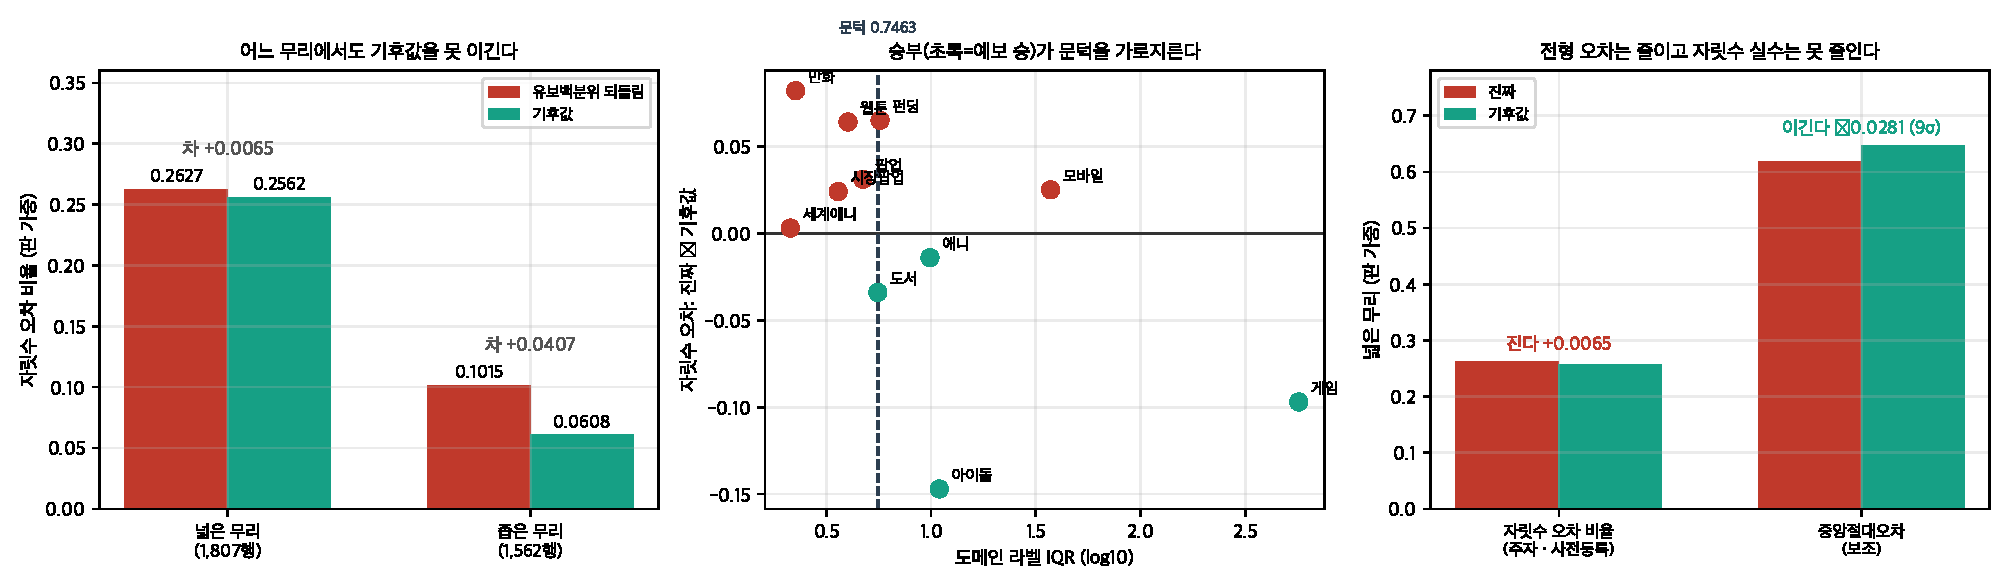
\includegraphics[width=0.99\textwidth]{figs/width.pdf}
\caption{왼쪽: 무리별 판 가중 --- 둘 다 기후값 승. 가운데: \textbf{승부가 문턱을
가로지른다} --- IQR 은 경계가 아니다. 오른쪽: 주자와 보조가 갈렸다.}
\end{figure}

\section{왜 무리 수준에서 뒤집혔나}

도메인별 승부는 논문 $159$ 그대로다 --- 게임($0.547 < 0.644$) · 아이돌($0.363 <
0.510$) · 애니 · 도서는 예보가 이긴다. \textbf{그런데 무리로 묶으면 진다.}

\begin{center}
\begin{tabular}{lrrl}
\toprule
넓은 무리 도메인 & 유보 행 & 자릿수(진짜 대 기후값) & \\
\midrule
게임 & $180$ & $0.547 < 0.644$ & 이긴다 \\
아이돌 & $51$ & $0.363 < 0.510$ & 이긴다 \\
애니 & $606$ & $0.136 < 0.150$ & 이긴다 \\
\textcolor{BrickRed}{모바일} & $441$ & $0.401 > 0.376$ & \textcolor{BrickRed}{진다} \\
\textcolor{BrickRed}{펀딩} & $529$ & $0.186 > 0.121$ & \textcolor{BrickRed}{진다} \\
\bottomrule
\end{tabular}
\end{center}

\claim{\textbf{도메인별 승부와 무리 가중 승부는 다른 것이다.} 펀딩 $529$행과
모바일 $441$행이 아이돌 $51$행과 게임 $180$행을 가중에서 누른다. 그리고
\textbf{승자였던 도서(IQR $0.746$)는 문턱 바로 아래로 떨어져 좁은 무리로 갔다.}
\textbf{라벨 넓이는 ``예보가 절대값에 값을 더하는 곳''의 경계가 아니다} ---
승자(게임·아이돌·애니·도서)와 패자(모바일·펀딩)가 IQR 축을 가로지른다.}
{무엇이 그 둘을 가르는지는 \textbf{모른다 --- 안 쟀다.} 후보 둘(예보 드리프트
크기 · 라벨 꼬리 비대칭)을 T$6$ 미결에 결정 규칙과 함께 적었다. $n{=}11$ 이라
스피어만 $|r| \geq 0.75$ 만 후보로 올린다.}

\subsection*{좁은 무리는 붙지 않았다 --- 기후값이 명확히 이긴다}

내 예측 ③은 \emph{``좁은 무리는 붙는다''}였다. 실측: 진짜 $0.1015$ 대 기후값
$\mathbf{0.0608}$ --- 차 $0.0407$, 잡음의 $10$배 밖. \textbf{라벨이 몰릴수록
기후값은 못 이기는 상대가 되는 정도가 아니라, 예보를 얹는 것이 명확히
해롭다}(만화 $0.090$ 대 $0.008$ --- $11$배).

\section{주자와 보조가 갈렸다}

\begin{center}
넓은 무리: 자릿수 오차 \textbf{진다}($+0.0065$) · 중앙절대오차 \textbf{이긴다}
($0.6187$ 대 $0.6468$ · $-0.0281$ · 잡음의 $9$배 밖)
\end{center}

\claim{\textbf{예보는 전형적 오차를 줄이고 자릿수 실수는 못 줄인다.} 사전등록이
자릿수 오차를 주자로 못박았으므로 \textbf{판정은 (나) 그대로다.} 중앙절대오차의
승리는 \emph{다른 질문}(``전형 오차 기준으로는 쓸모가 있나'')의 후보로만 적는다
--- 자를 바꿔 다시 묻는 것은 판정을 뒤집는 길이 아니다.}
{내 설계 실수 하나를 같이 적는다 --- \textbf{구간 덮음 비교가 공허했다.} 두 팔에
같은 기후값 구간을 줬으니 덮음이 정확히 같게($0.8655 = 0.8655$) 나온다. 논문
$159$ 의 구간 설계 실수를 피하려다 \textbf{비교 자체를 없앴다.} 예측 ④는 맞고
틀리고가 아니라 \textbf{시험이 없었다.}}

\section{처분}

능력 카드는 \textbf{안 바뀐다} --- 절대값 금지 그대로, 이제 \textbf{조건부 완화의
후보였던 길 하나가 정식으로 닫혔다.} 논문 $159$ 의 체리피킹 깃발은 이것으로
닫힌다: $4/11$ 은 실재하는 도메인별 사실이지만, \textbf{사전에 정한 어떤 라벨-넓이
규칙으로도 능력으로 승격되지 않는다.}

\begin{center}
T$6$ 의 다음 물음 --- \textbf{무엇이 승자와 패자를 가르나}(드리프트 크기 대 꼬리
비대칭 · 결정 규칙은 트랙에 적었다).
\end{center}

\end{document}
